\Group{Experiments}

\begin{frame}
    \frametitle{Data sets}
    \url{http://vision.ucsd.edu/~bbabenko/project_miltrack.html}
    \begin{itemize}
        \item 12 sequences
        \item 8 used in \cite{6126251}.
    \end{itemize}
\end{frame}

\begin{frame}
    \frametitle{Experimental Setup}
    \begin{itemize}
        \item Set up as described in their paper:
            \begin{itemize}
                \item Haar features
                \item Gaussian kernel with \(\sigma\) = 0.2
                \item \(C \in \{1, 2, ..., 100\}\)
                \item Search radius = 30 pixels
                \item SVM budget = 100
                \item Frame size = 320 x 240
                \item Random seed = 0
            \end{itemize}
    \end{itemize}
\end{frame}

\begin{frame}
    \frametitle{Scripting the Experiments}
    \begin{algorithm}[H]
        \DontPrintSemicolon
        \KwIn{Sequences}
        \Begin(Run experiments)
        {
            \ForEach{\(C \in \{1, 100\}\)}
            {
                \ForEach{Sequence}
                {
                    Update configuration file\;
                    Run Struck\;
                    Compare output with ground truth\;
                    Record mean IoU\;
                }
            }
        }
        \KwOut{IoU results}
    \end{algorithm}
\end{frame}

\begin{frame}
    \frametitle{Results}
    \begin{center}
        \begin{center}
%\begin{tabular}{l r r r}
%    \toprule
%    Sequence & Struck & \(s_{min}\) removal & no \(s_i = 0\) \\
%    \midrule
%    girl     &         0.681729  & \textbf{0.681821} & \textbf{0.681821} \\
%    surfer   &         0.787232  &         0.787232  & \textbf{0.811688} \\
%    tiger1   &         0.674713  &         0.651670  & \textbf{0.746060} \\
%    tiger2   &         0.667268  &         0.509582  & \textbf{0.679176} \\
%    twinings &         0.903097  & \textbf{0.931334} & \textbf{0.907482} \\
%    dollar   &         0.765203  &         0.765203  &         0.765203  \\
%    faceocc  &         0.853354  &         0.853354  &         0.853354  \\
%    cliffbar & \textbf{0.894553} &         0.890760  &         0.717940  \\
%    coke11   & \textbf{0.883395} &         0.882497  &         0.841359  \\
%    david    & \textbf{0.800847} &         0.434802  &         0.434802  \\
%    faceocc2 & \textbf{0.790128} &         0.789270  &         0.789270  \\
%    sylv     & \textbf{0.861525} &         0.857138  &         0.858211  \\
%    \bottomrule
%\end{tabular}

\begin{tabular}{l r r}
    \toprule
    Sequence & Struck & Fuzzy Struck \\
    \midrule
    girl     &         0.681729  & \textbf{0.681821} \\
    surfer   &         0.787232  & \textbf{0.811688} \\
    tiger1   &         0.674713  & \textbf{0.746060} \\
    tiger2   &         0.667268  & \textbf{0.679176} \\
    twinings &         0.903097  & \textbf{0.907482} \\
    dollar   &         0.765203  &         0.765203  \\
    faceocc  &         0.853354  &         0.853354  \\
    cliffbar & \textbf{0.894553} &         0.717940  \\
    coke11   & \textbf{0.883395} &         0.841359  \\
    david    & \textbf{0.800847} &         0.434802  \\
    faceocc2 & \textbf{0.790128} &         0.789270  \\
    sylv     & \textbf{0.861525} &         0.858211  \\
    \bottomrule
\end{tabular}
\end{center}

    \end{center}
\end{frame}

\begin{frame}
    \frametitle{Experimental Samples}
    \begin{columns}[T]
        \begin{column}{0.5\textwidth}
            \begin{figure}
                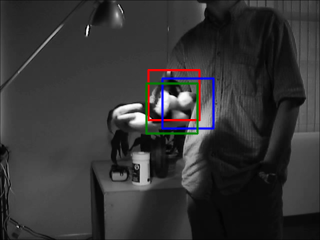
\includegraphics[width=0.9\textwidth]{sylv.png}
                \caption{Blue: Struck, Green: Fuzzy Struck}
            \end{figure}
        \end{column}
        \begin{column}{0.5\textwidth}
            \begin{figure}
                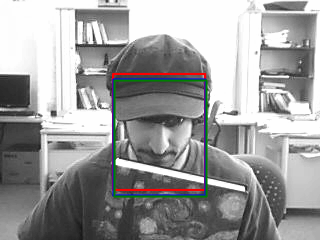
\includegraphics[width=0.9\textwidth]{faceocc2.png}
                \caption{Blue: Struck, Green: Fuzzy Struck}
            \end{figure}
        \end{column}
    \end{columns}
\end{frame}

\begin{frame}
    \frametitle{What else can be done?}
    \begin{itemize}
        \item Experiment with different fuzziness functions.
            \begin{itemize}
                \item Time: Calculate fuzziness based on current frame number.
                \item Velocity: Calculate fuzziness based on the target bounding box velocity.
            \end{itemize}
        \item Benchmark
            \begin{itemize}
                \item \url{http://alov300.org/}
                \item 314 sequences used in \cite{6671560}.
                \item Categorized to test various object tracking challenges.
                \item \alert{Haven't been successful downloading this data set!}
            \end{itemize}
    \end{itemize}
\end{frame}

%\begin{frame}
%    \frametitle{What went wrong?}
%    \begin{description}
%        \item [cliffbar] The target is lost when it is rotated about Y.
%        \item [coke11] The target is briefly lost when it is rotate about Z.
%        \item [david] Unknown
%        \item [faceocc2] Occluding object "pushes" the bounding box when the face is rotated.
%            Problem with feature vector orientation?
%    \end{description}
%\end{frame}

%\begin{frame}
%    \frametitle{Continous IoU}
%    \begin{center}
%        \includegraphics[height=0.8\textheight]{ious}
%    \end{center}
%\end{frame}
%
%\begin{frame}
%    \frametitle{Sample frame}
%    \begin{center}
%        \includegraphics[height=0.9\textheight]{tiger1_210}
%    \end{center}
%\end{frame}

